%==================== chapter2_2.tex ====================

\clearpage
\thispagestyle{plain}

\begingroup
\fontsize{16pt}{19.2pt}\selectfont
\justifying
\XeTeXlinebreakskip=0pt plus 1pt minus 0.5pt
\setlength{\parindent}{1.5cm}
\setlength{\parskip}{0pt}

\section*{Convolutional Neural Network (CNN)}
\addcontentsline{toc}{section}{Convolutional Neural Network (CNN)}

\ThaiPara{\cite{lecun1998gradient}~โครงข่ายประสาทเทียมแบบคอนโวลูชัน (Convolutional Neural Network: CNN)
	ถูกออกแบบมาเพื่อจัดการข้อมูลที่มีโครงสร้างพื้นที่ เช่น รูปภาพ หัวใจคือชั้นคอนโวลูชันซึ่งใช้ฟิลเตอร์
	(kernel) เลื่อนไปบนภาพเพื่อสกัดคุณลักษณะ (เช่น ขอบและลวดลาย) ทำให้จำนวนพารามิเตอร์ลดลง
	และคำนวณได้มีประสิทธิภาพ นอกจากนี้ยังมีแนวคิด \emph{padding} เพื่อคงขนาดข้อมูล
	\emph{stride} เพื่อกำหนดก้าวการเลื่อนฟิลเตอร์ และชั้น \emph{pooling} (เช่น \emph{max pooling})
	เพื่อลดขนาดข้อมูล ก่อนส่งต่อไปยังชั้นเชื่อมต่อสมบูรณ์และ \emph{softmax} เพื่อจำแนกประเภท}

\vspace{\baselineskip}

% คำบรรยายรูปให้ justified เฉพาะรูปนี้
\begin{figure}[h]
	\centering
	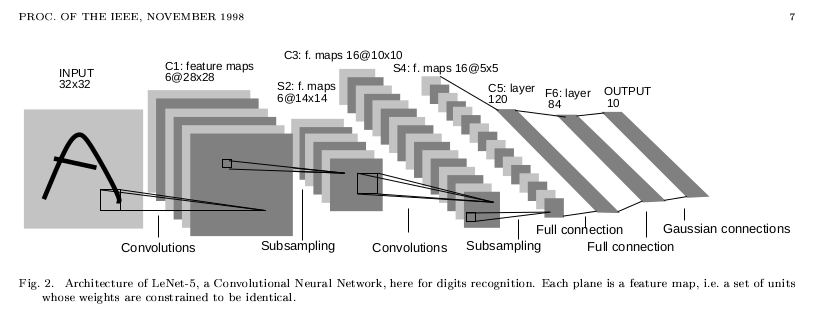
\includegraphics[width=0.8\linewidth]{ml-blog19-lenet5}
	\caption{สถาปัตยกรรมพื้นฐานของ Convolutional Neural Network (CNN)}
\end{figure}



\section*{Image classification (การจำแนกภาพ)}
\addcontentsline{toc}{section}{Image classification (การจำแนกภาพ)}

% ---------- Image classification ----------
\noindent{\bfseries\fontsize{16pt}{19.2pt}\selectfont }\par

\ThaiPara{\cite{superannotate2023imageclassification}~การจำแนกภาพคือการกำหนดป้ายกำกับให้รูปภาพจากชุดป้ายที่กำหนดล่วงหน้า
	ปัจจุบันโมเดลเชิงลึก โดยเฉพาะ CNN สามารถเรียนรู้คุณลักษณะสำคัญจากพิกเซลดิบแบบปลายทางถึงปลายทาง
	(\emph{end-to-end}) และส่งออกค่าความน่าจะเป็นของแต่ละคลาสได้อย่างมีประสิทธิภาพ}

\vspace{\baselineskip}

\begin{figure}[h]
	\centering
	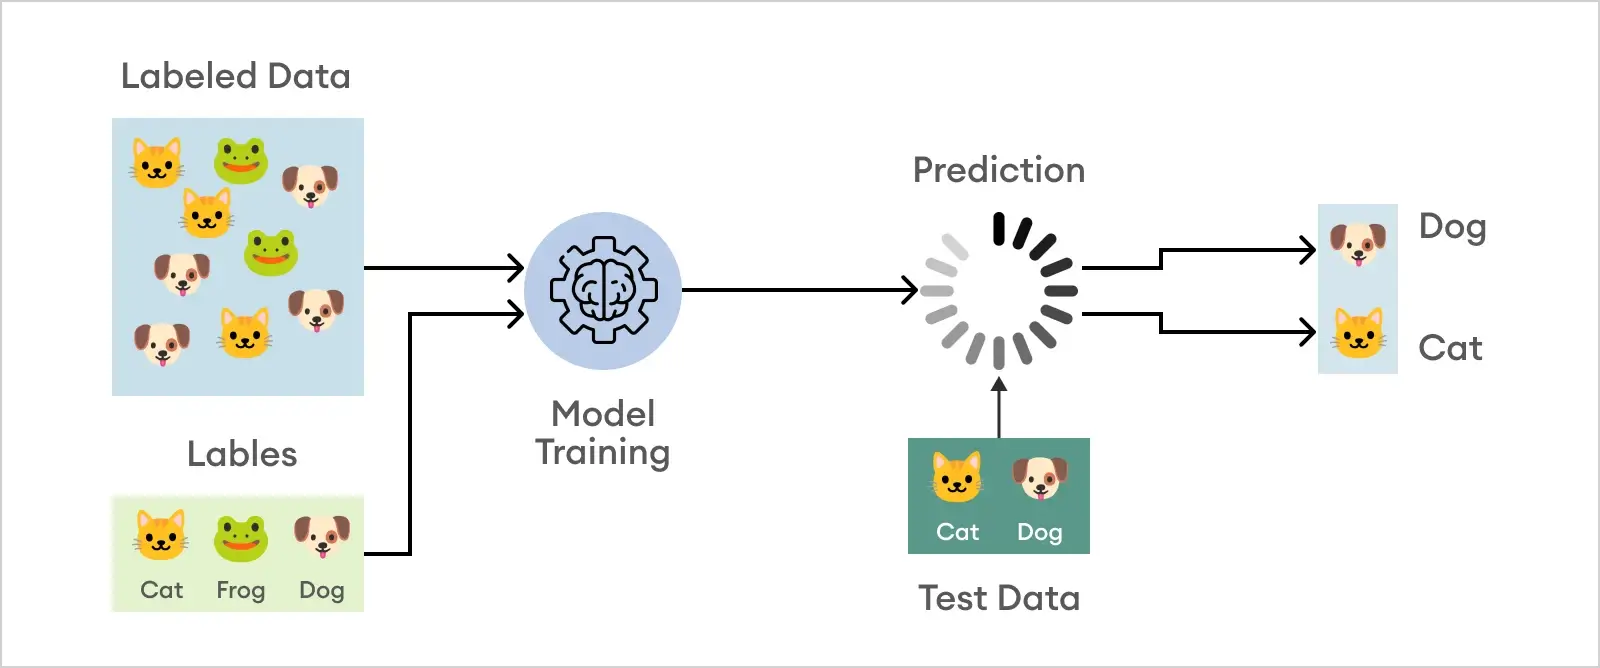
\includegraphics[width=0.8\linewidth]{png1}
	\caption{สถาปัตยกรรมพื้นฐานของการจำแนกภาพ}
\end{figure}

\par\endgroup
\clearpage
%================== จบ chapter2_1.tex ====================
